\documentclass[10pt]{scrartcl}

\usepackage{abstract}

\usepackage[utf8]{inputenc}

\usepackage{tabularx}

\usepackage{amsmath}
\usepackage{amssymb}
% rand
\usepackage{geometry}
\geometry{a4paper, top=25mm, left=30mm, right=25mm, bottom=30mm,
         headsep=10mm, footskip=12mm}

\usepackage{graphicx}
\usepackage{url}

\usepackage{graphicx}
\usepackage[pdftex,colorlinks=true,citecolor=blue,urlcolor=blue,linkcolor=blue]{hyperref}


\usepackage{color}
\usepackage{xcolor}

\usepackage{tabularx}

\usepackage{amsmath}
\usepackage{amssymb}
%\usepackage{lscape}
%\usepackage{ragged2e}

\usepackage{listings}

\usepackage[margin=10pt]{caption}

\newtheorem{definition}{Definition}


\author{Philipp Wagner\thanks{\url{http://www.bytefish.de}, bytefish--at--gmx--dot--de}}
\title{Statistical Machine Learning with OpenCV}
%\date{Wintersemester 2010}

\RequirePackage{listings}
\lstdefinelanguage{pseudocode}{
morekeywords=[1]{procedure, while, do, endwhile},
morecomment=[l]{\%}
}

\lstset{%
	frame=lines,
	columns=fullflexible
}

\definecolor{darkblue}{rgb}{0,0,.6}
\definecolor{darkred}{rgb}{.6,0,0}
\definecolor{darkgreen}{rgb}{0,.6,0}
\definecolor{red}{rgb}{.98,0,0}

\lstloadlanguages{C++}
\lstset{%
  language=C++,
  basicstyle=\tiny\sffamily,
  commentstyle=\itshape\color{darkgreen},
  keywordstyle=\bfseries\color{darkblue},
  stringstyle=\color{darkred},
  frame=lines,
  columns=fullflexible,
  showspaces=false
}%

% redefine lstinline
\makeatletter
\lst@AddToHook{TextStyle}{\let\lst@basicstyle\normalsize\sffamily}
\makeatother

% change vertical space of itemize and enumeration environments
\let\olditemize=\itemize
   \def\itemize{\olditemize\setlength{\itemsep}{-0.5ex}}
\let\oldenumerate=\enumerate
   \def\enumerate{\oldenumerate\setlength{\itemsep}{-0.5ex}}


\begin{document}

\maketitle

% abstract info
\begin{abstract}
This document is an introduction to Machine Learning with OpenCV. Artificial Neural Networks and Support Vector Machines are briefly explained and examples in OpenCV are given.
\end{abstract}

% include sections
\section{Introduction}

This document covers the Machine Learning API of the OpenCV2 C++ API. It helps you with setting up your system, gives a brief introduction into Support Vector Machines and Neural Networks and shows how it's implemented with OpenCV. Machine Learning is a branch of Artificial Intelligence and concerned with the question how to make machines able to learn from data. The core idea is to enable a machine to make intelligent decisions and predictions, based on experiences from the past. Algorithms of Machine Learning require interdisciplinary knowledge and often intersect with topics of statistics, mathematics, physics, pattern recognition and more.

\href{http://opencv.willowgarage.com}{OpenCV2} comes with a machine learning library for:
\begin{itemize}
 \item Decision Trees
 \item Boosting
 \item Support Vector Machines
 \item Expectation Maximization
 \item Neural Networks
\end{itemize}

\href{http://opencv.willowgarage.com}{OpenCV (Open Source Computer Vision)} is a popular computer vision library started by \href{http://www.intel.com}{Intel} in 1999. The cross-platform library sets its focus on real-time image processing and includes patent-free implementations of the latest computer vision algorithms. In 2008 \href{http://www.willowgarage.com}{Willow Garage} took over support and OpenCV 2.3.1 now comes with a programming interface to C, C++, \href{http://www.python.org}{Python} and \href{http://www.android.com}{Android}. OpenCV is released under a BSD license, so it is used in academic and commercial projects such as \href{http://www.google.com/streetview}{Google Streetview}.

Please don't copy and paste the code from this document, the project has been uploaded to \url{http://www.github.com/bytefish/opencv}. All code is released under a \href{http://www.opensource.org/licenses/bsd-license}{BSD license}, so feel free to use it for your projects.

\section{Setup}
Follow this guide to have a Development Environment for Linux and Windows. You have to download Eclipse and CMake. Windows users can use MinGW as a C/C++ compiler. 

\subsection{Eclipse with CDT (Windows/Linux)}
Eclipse is an Integrated Development Environment (IDE). It is possibly best known as a Java development platform, but can be extended for languages such as C/C++, PHP, Python and more. The easiest way to get Eclipse with C/C++ support is to download \textit{Eclipse for C++ Developers} for your operating system at: \url{http://www.eclipse.org/downloads/}. The download already includes the CDT Plugin (C/C++ Development Toolkit).

There is no installation. Just unpack and start the eclipse executable.

\subsection{MinGW (Windows only)}
This step is Windows only. \htmladdnormallink{MinGW (Minimalist GNU for Windows)}{http://www.mingw.org} is a port of the \htmladdnormallink{GNU Compiler Collection (GCC)}{http://gcc.gnu.org} and can be used for development of native \htmladdnormallink{Microsoft Windows}{http://www.microsoft.com/windows} applications. Download the automated mingw-get-installer \htmladdnormallink{from sourceforge}{http://sourceforge.net/projects/mingw/files/Automated\%20MinGW\%20Installer/mingw-get-inst/} (called \textit{mingw-get-inst-20101030.exe} at time of writing this). If the path to the download changes, navigate there from the MinGW project page at: \url{http://www.mingw.org}. Be sure to select \textit{"C++ Compiler"} in the \textit{Compiler Suite} dialog during setup.

MinGW doesn't add its binaries to the global Windows PATH environment. The MinGW Page says: \textit{Add }\verb|C:\MinGW\bin;|\textit{ to the PATH environment variable by opening the System control panel, going to the Advanced tab, and clicking the Environment Variables button. If you currently have a Command Prompt window open, it will not recognize the change to the environment variables; you will need to open a new Command Prompt window to get the new PATH.}

\subsection{CMake}
\htmladdnormallink{CMake}{http://www.cmake.org} is an open-source, cross-platform build system used by many opensource projects including: \htmladdnormallink{OpenCV}{http://opencv.willowgarage.com}, \htmladdnormallink{MiKTeX}{http://www.miktex.org} or \htmladdnormallink{Blender 3D}{http://www.blender.org}. It works on Linux, Windows, Mac OS X and can generate (among many others) Eclipse CDT project files and that's why it is suggested as a build system for OpenCV projects.

\subsubsection*{Windows} 
Download the installer from the \htmladdnormallink{Resources Page}{http://www.cmake.org/cmake/resources/software.html} at \url{http://www.cmake.org} (called cmake-2.8.3-win32-x86.exe at time of writing). This will install cmake, ccmake and the cmake-gui.

Make sure to select \textit{"Add CMake to the system PATH for all users"} during setup.

\subsubsection*{Linux}
CMake is often available from a distributions repository or can be downloaded as an installer from the \htmladdnormallink{Resources Page}{http://www.cmake.org/cmake/resources/software.html} at \url{http://www.cmake.org}. Installing the generic Linux binaries with the is done by typing:
\begin{lstlisting}
sudo sh cmake-2.8.3-Linux-i386.sh --prefix=/usr/local 
\end{lstlisting}

In Debian or Ubuntu cmake can be installed with apt:
\begin{lstlisting}
sudo apt-get install cmake cmake-gui
\end{lstlisting}


\subsection{OpenCV}
\htmladdnormallink{OpenCV}{http://opencv.willowgarage.com} is a Computer Vision Library started by \htmladdnormallink{Intel}{http://www.intel.com} in 1999 and now actively developed by \htmladdnormallink{Willow Garage}{http://www.willowgarage.com}. It includes advanced computer vision algorithms and sets the focus on real-time image processing. In 2009 OpenCV2 got a C++ interface and integrates with Python. If you encounter any problems with this install guide consult the \htmladdnormallink{OpenCV Install Guide}{http://opencv.willowgarage.com/wiki/InstallGuide} aswell.
 
\subsubsection*{Windows}
\htmladdnormallink{Mircosoft Windows}{http://www.microsoft.com/windows} users download the Windows installer from the sourceforge repository of OpenCV at \url{http://sourceforge.net/projects/opencvlibrary/}. (called \htmladdnormallink{OpenCV-2.2.0-win32-vs2010.exe}{http://sourceforge.net/projects/opencvlibrary/files/opencv-win/2.2/} at time of writing this). 

Make sure to select \textit{"Add OpenCV to the system PATH for all users"} during setup.

\subsubsection*{Linux}
Linux users should inspect their repositories, because most distributions have pre-packaged binaries. In Debian/Ubuntu you simply type:
\begin{lstlisting}
sudo apt-get install opencv opencv-doc
\end{lstlisting}

\subsubsection*{Build OpenCV from sources}
OpenCV is open source and comes with CMake as build system. Sometimes you need to compile OpenCV yourself, for example if the pre-packaged binaries use SSE2 and your CPU doesn't support SSE2. If so, download the OpenCV sources, unpack them and cd to the directory.

For building OpenCV from source type:
\begin{lstlisting}
cmake .
make 
sudo make install
\end{lstlisting}

\subsubsection*{Building OpenCV without SSE2}
If you are actually working on a CPU without SSE2 you will need to deselect the SSE2 build option before compiling it, otherwise OpenCV won't work as expected. To see which flags your CPU supports (assuming Linux), type \lstinline{cat /proc/cpuinfo | grep flags} in a terminal.

On my workstation:

\begin{lstlisting}
philipp@banana:~$ cat /proc/cpuinfo | grep flags
flags           : fpu vme de pse tsc msr pae mce cx8 sep mtrr pge mca cmov pat pse36 mmx fxsr sse syscall mp mmxext 3dnowext 3dnow up ts fid vid
\end{lstlisting}

It's an \htmladdnormallink{AMD}{http://www.amd.com} Athlon XP and does not support SSE2. In order to turn off SSE2 support for OpenCV with the cmake-gui:
\begin{itemize}
\item Start \texttt{cmake-gui} either from prompt or menu.
\item Set the OpenCV source folder as \textit{Source Directory} and \textit{Build Directory}
\item Click \textit{configure} and choose: \texttt{Unix Makefiles}.
\item Deselect \textit{ENABLE\_SSE2} support from the list of flags.
\item Click \textit{configure} again to accept the setup.
\item Click \textit{generate} and proceed with the normal compiling procedure as described above.
\end{itemize}

The command line for doing the same would be (assuming you are in the OpenCV folder):

\begin{lstlisting}
cmake -DENABLE_SSE2=OFF .
\end{lstlisting}
followed by:
\begin{lstlisting}
make
sudo make install
\end{lstlisting}


% 
% \section{Getting started with CMake}
% This chapter serves as an introduction to CMake, because it is used for the OpenCV project. Instead of making up a simple Hello World, it will show how to write, test and build a library with CMake and the \htmladdnormallink{Boost Framework}{http://www.boost.org}.
% \subsection*{Problem}
% Imagine your are working on a project with GPS data and you are told to write and test a library, let's call it \textit{geolib}, to calculate the distance between two positions on earth (also called great-circle distance or orthodromic distance). Points on earth are given in latitude ($\phi$) and longitude ($\lambda$) and for the distance calculation one can use the haversine formula:
% \begin{equation}
% \label{eq:haversine}
% \operatorname{haversin}\left(\frac{d}{R}\right) = \operatorname{haversin}(\varphi_2 - \varphi_1) + \cos(\varphi_1) \cos(\varphi_2)\,\operatorname{haversin}(\Delta\lambda).
% \end{equation}
% 
% Where $haversin$ is:
% 
% \begin{displaymath}
% haversin(\theta) = \sin^2 (\theta / 2)
% \end{displaymath}
% 
% And applying the inverse haversine gives the distance $d$:
% 
% \begin{displaymath}
% d = R \, \operatorname{haversin}^{-1}(h) = 2 R \arcsin\left(\sqrt{h}\,\right)
% \end{displaymath}
%  
% Where $h$ is:
% \begin{displaymath}
% h =  \operatorname{haversin}(\frac{d}{R})
% \end{displaymath}
% 
% \subsection*{Files}
% The final project has a structure shown in Listing \ref{lst:cmake_files}. The source files are in the appendix or can be downloaded from: \url{http://bytefish.de/lib/exe/fetch.php?media=blog:cmake_example.zip}.
% 
% \begin{lstlisting}[label=lst:cmake_files, caption=Project structure.]
% philipp@banana:~/git/cmake$ tree src
% src/
% |-- CMakeLists.txt
% |-- geolib
% |   |-- geolib.cc
% |   |-- geolib.h
% |   `-- test.cc
% `-- main.cc
% 
% 1 directory, 5 files
% \end{lstlisting}
% 
% 
% \subsection*{Implementation}
% 
% You start by implementing the library. The header file in Listing \ref{lst:geolib.h} is using \htmladdnormallink{Doxygen}{http://www.stack.nl/~dimitri/doxygen/} annotations to document the code. Doxygen is not introduced here, but it is strongly advised to document your work (because someone wants to \textit{use} and \textit{understand} it aswell). The corresponding source file in Listing \ref{geolib.cc} implements the haversine formula given in equation \ref{eq:haversine}.
% 
% \begin{lstlisting}[language=C++, label=lst:geolib.h, caption=lst:geolib.h]
% #ifndef _geolib_h
% #define _geolib_h
% #include <math.h>
%  
% /**
% * @author philipp
% * @date 2010
% */
% namespace geolib {
%  
%     const double DEG2RAD = M_PI / 180.0;
%     const double RAD2DEG = 180.0 / M_PI;
%     const double EARTH_RADIUS = 6371.01;
%  
%     /**
%      * @brief great-circle distance (shortest distance between two points on earth)
%      * @param[in] latitude point 1
%      * @param[in] longitude point 1
%      * @param[in] latitude point 2
%      * @param[in] longitude point 2
%      * @return great-circle distance
%     */
%     double great_circle_distance(double lat1, double long1, double lat2, double long2);
%  
% }
%  
% #endif
% \end{lstlisting}
% The corresponding source file in geolib.cc implements the haversine formula given in the projects description: 
% \begin{lstlisting}[language=C++, label=lst:geometry.cc, caption=geometry.cc]
% #include "geolib.h"
%  
% namespace geolib {
%  
%     double great_circle_distance(double lat1, double long1, double lat2, double long2) {
%         lat1 *= DEG2RAD;
%         long1 *= DEG2RAD;
%         lat2 *= DEG2RAD;
%         long2 *= DEG2RAD;
%  
%         double deltaLat = lat1-lat2;
%         double deltaLong = long1-long2;
%         double a = pow(sin(deltaLat/2.0),2.0) + cos(lat1) * cos(lat2) * pow(sin(deltaLong/2.0),2.0);
%         double c = 2 * asin(sqrt(a));
%  
%         return EARTH_RADIUS * c;
%     }
%  
% }
% \end{lstlisting}
% 
% \subsection{Tests}
% Software has bugs. So tests are important in software development to ensure that components are working correctly. They are a sort of living documentation and should reduce defects and failures, especially when refactoring software. If you are used to JUnit you will find the Boost unit testing framework for C++ pleasing. Boost (\url{http://www.boost.org}) is a great library that adds enormous extra power to C++.
% 
% The Boost testing framework is a set of macros to validate expressions and each macro belongs to one of the three warning levels:
% \begin{itemize}
%  \item \textbf{WARN} logs a warning if the test fails
%  \item \textbf{CHECK} continues the test on failure
%  \item \textbf{REQUIRE} stops the test on failure
% \end{itemize}
% 
% The best introduction is probably given by \htmladdnormallink{IBM developerWorks: Get to know the Boost unit test framework}{http://www.ibm.com/developerworks/aix/library/au-ctools1_boost/}. A list of available macros is given by the \htmladdnormallink{Boost documentation on testing tools}{http://www.boost.org/doc/libs/1_45_0/libs/test/doc/html/utf/testing-tools/reference.html}
% Listing \ref{lst:test.cc} shows how to test the great-circle distance of the geolib with the Boost unit testing framework. As test data I use the airport example from the Wikipedia Page on Great-circle distance: 
% 
% \begin{lstlisting}[language=C++, label=lst:test.cc, caption=test.cc]
% #define BOOST_TEST_DYN_LINK
% #define BOOST_TEST_MODULE "GeoLib Tests"
% #include <boost/test/unit_test.hpp>
% #include "geolib.h"
% 
% BOOST_AUTO_TEST_CASE(gcircle_test) {
% 
% 	double expected = 2886.448973436;
% 
% 	double bna_lat = 36.12;
% 	double bna_long = -86.67;
% 	double lax_lat = 33.94;
% 	double lax_long = -118.40;
% 
% 	double actual = geolib::great_circle_distance(bna_lat, bna_long, lax_lat, lax_long);
% 	BOOST_CHECK_CLOSE(expected, actual, 1e-5);
% 
% }
% 
% \end{lstlisting}
% 
% 
% \subsection{CMakeLists.txt: Putting it all together}
% CMake searches for a file called \textit{CMakeLists.txt} in a given directory. The CMakeLists.txt for this project is: 
% 
% \begin{lstlisting}[label=lst:CMakeLists.txt, caption=CMakeLists.txt]
% CMAKE_MINIMUM_REQUIRED( VERSION 2.6 )
% PROJECT(HELLOWORLD_PROJECT)
% INCLUDE_DIRECTORIES("${CMAKE_SOURCE_DIR}/geolib")
% ADD_LIBRARY(geolib geolib/geolib.cc geolib/geolib.h)
% ADD_EXECUTABLE(helloworld main.cc)
% TARGET_LINK_LIBRARIES(helloworld geolib)
% 
% # Tests
% FIND_PACKAGE( Boost REQUIRED COMPONENTS unit_test_framework)
% INCLUDE_DIRECTORIES(${Boost_INCLUDE_DIRS})
% ADD_EXECUTABLE(test_geolib geolib/test.cc)
% TARGET_LINK_LIBRARIES(test_geolib ${Boost_LIBRARIES} geolib)
% \end{lstlisting}
% 
% \subsection{Build}
% Building the project can be done by an out of source build: 
% \begin{lstlisting}
% philipp@banana:~/git/cmake$ mkdir build && cd build
% philipp@banana:~/git/cmake/build$ cmake ../src/
% philipp@banana:~/git/cmake/build$ make
% \end{lstlisting}
% Running the executable \textit{helloworld} calculates the distance from Berlin to Munich (in km):
% \begin{lstlisting}
% philipp@banana:~/git/cmake/build$ ./helloworld
% Distance is 508.978.
% \end{lstlisting}
% Running the test returns no errors:
% \begin{lstlisting}
% philipp@banana:~/git/cmake/build$ ./test_geolib
% Running 1 test case...
% 
% *** No errors detected
% \end{lstlisting}

\section{Getting Started with OpenCV}
Now that Eclipse, MinGW (Windows), CMake and OpenCV are installed it is time to create the first OpenCV project. It is called \textit{hello\_opencv}. Files for this example are put in a folder at: \verb|C:\workspace\hello_opencv|. Of course any valid path can be chosen and kept consistent with the example.

\subsubsection*{1. CMakeLists.txt}
CMake searches for a file called CMakeLists.txt The OpenCV library is linked against the executable. Save CMakeLists.txt from Listing \ref{lst:cmakelists.txt} to \verb|C:\workspace\hello_opencv|.
 
\begin{lstlisting}[caption=CMakeLists.txt, label=lst:cmakelists.txt]
cmake_minimum_required(VERSION 2.6)
PROJECT(hello_opencv_proj)
FIND_PACKAGE( OpenCV REQUIRED )
ADD_EXECUTABLE( hello_opencv main.cpp)
TARGET_LINK_LIBRARIES( hello_opencv ${OpenCV_LIBS} )
\end{lstlisting}

\subsubsection*{2. main.cpp}
Now the OpenCV C++ API is introduced.

\begin{lstlisting}[language=C++, label=lst:main.cpp]
#include "cv.h"
#include "ml.h"

using namespace std;

int main() {
	cv::Mat plot(240,320,CV_8UC3);
	plot.setTo(cv::Scalar(255,255,255));
	cv::putText(plot,"Hello OpenCV",Point(1,100), FONT_HERSHEY_SIMPLEX, 1.0 ,Scalar(0,0,0), 1, 8, false);
	cv::namedWindow("Hello OpenCV", CV_WINDOW_AUTOSIZE);
	cv::imshow("Hello OpenCV", plot);
	cv::waitKey();
}
\end{lstlisting}

Save main.cpp from Listing \ref{lst:main.cpp} to \verb|C:\workspace\hello_opencv|.

\subsubsection*{3. Generate project and makefiles}
We will need to import the project to eclipse, so we generate the CDT specific Makefiles:

\begin{itemize}
\item Start the \textit{cmake-gui}
\item Browse to \verb|C:\workspace\hello_opencv| as \textit{Source Folder} and \textit{Build Folder}
\item Click \textit{configure} and select "Eclipse CDT4 - Unix Makefiles" from the Dialog
\item Click \textit{configure} again to accept the configuration
\item Click \textit{generate} to generate the Makefiles and Eclipse related project files
\end{itemize}

Your folder will now look like this:

\begin{lstlisting}
C:\workspace\hello_opencv>dir

11.12.2010  14:33    <DIR>          .
11.12.2010  14:33    <DIR>          ..
11.12.2010  14:33            22.202 .cproject
11.12.2010  14:33             3.591 .project
11.12.2010  14:28            29.062 CMakeCache.txt
11.12.2010  14:33    <DIR>          CMakeFiles
11.12.2010  14:18               190 CMakeLists.txt
11.12.2010  14:28             1.470 cmake_install.cmake
11.12.2010  14:14               556 main.cpp
11.12.2010  14:33             5.179 Makefile
\end{lstlisting}

If you feel more familiar with a terminal type:

\begin{lstlisting}
C:\> cd C:\workspace\hello_opencv
C:\> cmake -G"Eclipse CDT4 - Unix Makefiles" .
\end{lstlisting}

\subsubsection*{4. Import project and makefiles into Eclipse}
Start Eclipse and from the menu choose:
\begin{enumerate}
 \item \verb|File -> Import...|
 \item \verb|General -> Existing Projects into Workspace|
 \item Select \verb|C:\workspace\hello_opencv| as root directory
 \item Click \verb|Finish|
\end{enumerate}

\subsubsection*{5. Build and run the project}
To build the project:
 \begin{itemize}
  \item \verb|Project -> Build All|
 \end{itemize}
To run the project:
\begin{itemize}
 \item \verb|Run -> Run|
\end{itemize}

And a window similar to Figure \ref{fig:helloworld} pops up.

\begin{figure}[ht!]
\label{fig:helloworld}
\caption{OpenCV: Hello World}
 \begin{center}
   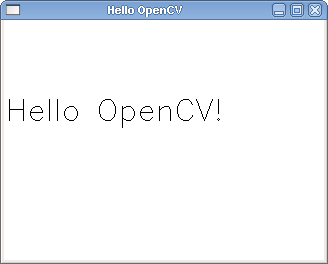
\includegraphics[scale=0.5]{img/helloopencv.png}
 \end{center}
\end{figure}
\section{Random Numbers in OpenCV}
Each thread in OpenCV has access to a default random number generator \lstinline|cv::theRNG()|. For a single pass the seed for the random number generator doesn't have to be set, but if many random numbers have to be generated (for example in a loop) the seed has to be set.

This can be done by assigning the local time to the random number generator:

\begin{lstlisting}
 cv::theRNG() = cv::RNG(time(0))
\end{lstlisting}

\subsection{Uniform Distribution}
Uniform Distributions can be generated in OpenCV with the help of \textit{cv::randu}. The signature of \textit{cv::randu} is:
\begin{lstlisting}[language=C++]
void randu(Mat& mtx, const Scalar& low, const Scalar& high);
\end{lstlisting}
Where
\begin{itemize}
 \item \textbf{mtx} is the Matrix to be filled with uniform distributed random numbers
 \item \textbf{low} is the inclusive lower boundary of generated random numbers
 \item \textbf{high} is the exclusive upper boundary of generated random numbers
\end{itemize}


\subsection{Normal Distribution}
Normal Distribution can be generated in OpenCv with the help of \textit{cv::randn}.
\begin{lstlisting}[language=C++]
void randn(Mat& mtx, const Scalar& mean, const Scalar& stddev);
\end{lstlisting}
Where
\begin{itemize}
 \item \textbf{mtx} is the Matrix to be filled with normal distributed random numbers
 \item \textbf{mean} the mean value of the generated random numbers
 \item \textbf{stddev} the standard deviation of the generated random numbers
\end{itemize}

\subsection{Bivariate Gaussian Distribution}

Multivariate normal distributions can be generated with the C API by using \textit{cvRandMVNormal} from the Machine Learning library. However this function seems to have no C++ equivalent yet, so in order to generate random numbers for the bivariate case one can also use the function given in \ref{lst:bivar}.

\begin{lstlisting}[language=C++, caption=bivariate\_gaussian dstribution, label=lst:bivar]
void bivariate_gaussian(float mu_x, float sigma_x, float mu_y, float sigma_y, float rho, cv::Mat &x, cv::Mat &y) {
  assert(x.rows == y.rows && x.rows > 0);

  int n = x.rows;

  randn(x, mu_x, sigma_x);

  cv::Mat r(n,1, CV_32FC1);
  cv::theRNG() = cv::RNG(time(0));

  randn(r, 0, 1);
  for(int i = 0; i < n; i++) {
    y.at<float>(i, 0) = sqrt(sigma_y*sigma_y - (rho * sigma_y)*(rho * sigma_y)) * r.at<float>(i, 0) + mu_y;
    y.at<float>(i, 0) = y.at<float>(i,0) + rho * sigma_y/sigma_x * (x.at<float>(i,0) - mu_x);
}
\end{lstlisting}


\section{Preparing the Training and Test Dataset for OpenCV ML}
In the C++ Machine Learning API of OpenCV training and test data is given as a \lstinline|cv::Mat| matrix. The constructor of \lstinline|cv::Mat| is defined as:
\begin{lstlisting}[language=C++]
Mat::Mat(int rows, int cols, int type);
\end{lstlisting}
Where
\begin{itemize}
 \item rows is the number of samples (for all classes!)
 \item columns is the number of dimensions
 \item type is the image type
\end{itemize}

In the machine learning library of OpenCV each row or column in the training data is a n-dimensional sample. The default ordering is row sampling and class labels are given in a matrix with equal length (one column only, of course). 

\begin{lstlisting}[language=C++]
cv::Mat trainingData(numTrainingPoints, 2, CV_32FC1);
cv::Mat testData(numTestPoints, 2, CV_32FC1);

cv::randu(trainingData,0,1);
cv::randu(testData,0,1);

cv::Mat trainingClasses = labelData(trainingData, equation);
cv::Mat testClasses = labelData(testData, equation);
\end{lstlisting}

Since only binary classification problems are considered the function \lstinline|f| returns the classes $-1$ and $1$ for a given two-dimensional data point:

\begin{lstlisting}[language=C++]
// function to learn
int f(float x, float y, int equation) {
  switch(equation) {
  case 0:
    return y > sin(x*10) ? -1 : 1;
    break;
  case 1:
    return y > cos(x * 10) ? -1 : 1;
    break;
  case 2:
    return y > 2*x ? -1 : 1;
    break;
  case 3:
    return y > tan(x*10) ? -1 : 1;
    break;
  default:
    return y > cos(x*10) ? -1 : 1;
  }
}
\end{lstlisting}

And to label data one can use the function \lstinline|labelData|:
\begin{lstlisting}
cv::Mat labelData(cv::Mat points, int equation) {
  cv::Mat labels(points.rows, 1, CV_32FC1);
  for(int i = 0; i < points.rows; i++) {
    float x = points.at<float>(i,0);
    float y = points.at<float>(i,1);
    labels.at<float>(i, 0) = f(x, y, equation);
  }
  return labels;
}
\end{lstlisting}
\section{Support Vector Machines (SVM)}
Support Vector Machines were first introduced by Vapnik and Chervonenkis in \cite{VC74}. The core idea is to find the optimal hyperplane to seperate a dataset, while there are theoretically infinite hyperplanes to seperate the dataset. A hyperplane is chosen, so that the distance to the nearest datapoint of both classes is maximized (Figure \ref{fig:maximum_margin}). The points spanning the hyperplane are the \textit{Support Vectors}, hence the name \textit{Support Vector Machines}. \cite{VC95}

\begin{figure}
\begin{center}
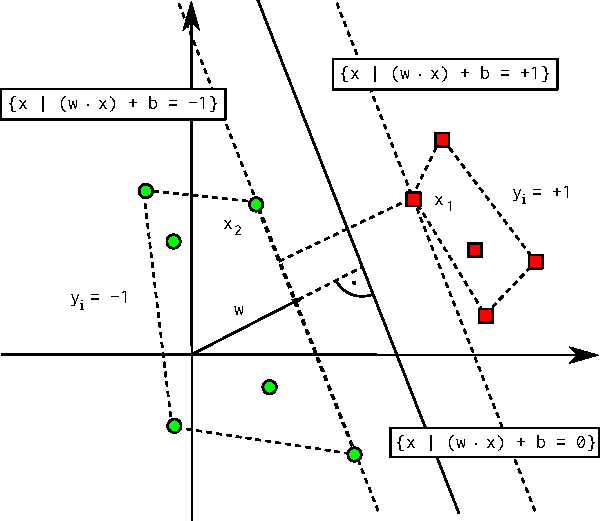
\includegraphics[scale=0.7]{img/svm/margin.pdf}
 % margin.pdf: 289x250 pixel, 72dpi, 10.20x8.82 cm, bb=0 0 289 250
\end{center}
 \caption{Maxmimum Margin Classifier.}
 \label{fig:maximum_margin}
\end{figure}

\subsection{Definition}
Given a Set of Datapoints $\mathcal{D}$:

$$\mathcal{D} = \left\{(x_i, y_i) | x_i \in \mathbb{R}^p, y_i \in \left\{-1,1\right\}\right\}_{i=1}^n$$
where
\begin{itemize}
 \item $x_i$ is a point in p-dimensional vector
 \item $y_i$ is the corresponding class label
\end{itemize}
We search for $\omega \in \mathbb{R}^n$ and bias $b$, forming the Hyperplane H:
$$\omega^T x + b = 0$$
that seperates both classes so that:
$$ \omega^T x + b = 1,\mbox{if } y = 1 $$
$$ \omega^T x + b = -1, \mbox{if } y = -1 $$

The optimization problem that needs to be solved is:
$$\mbox{min } \frac{1}{2}\omega^T \omega$$
subject to:
$$\omega^T x + b \geq 1, y = 1$$
$$\omega^T x + b \leq 1, y = -1 $$

Such quadratic optimization problems can be solved with standard solvers, such as \htmladdnormallink{GNU Octave}{www.gnu.org/software/octave} or \htmladdnormallink{Matlab}{www.mathworks.com/products/matlab}.

\subsubsection{Non-linear SVM}
The kernel trick is used for classifying non-linear datasets. It works by transforming data points into a higher dimensional feature space with a \textit{kernel function}, where the dataset can be seperated again (see Figure \ref{fig:kernel_trick}).


\begin{figure}[ht!]
\begin{center}
 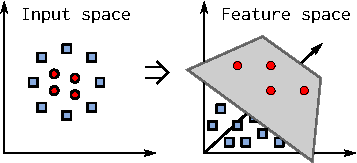
\includegraphics[scale=1.3]{img/svm/input_space2.pdf}
 \caption{Kernel Trick}
 \label{fig:kernel_trick}
 % input_space2.pdf: 1179666x1179666 pixel, 0dpi, infxinf cm, bb=
\end{center}
\end{figure}


Commonly used kernel functions are \textit{RBF kernels}:
$$k(x,x') = exp(\frac{\|x-x'\|^2}{\sigma^2})$$ 
or \textit{polynomial kernels}:
$$k(x,x') = (x \cdot x')^d$$.



\subsection{SVM in OpenCV}
Parameters for a SVM have to be defined in the structure \textit{CvSVMParams}.

\subsubsection*{Parameters}
\begin{lstlisting}[language=C++, caption=Example CvSVMParams, label=lst:cvsvmparams]
CvSVMParams param = CvSVMParams();

param.svm_type = CvSVM::C_SVC;
param.kernel_type = CvSVM::LINEAR;

param.degree = 0; // for poly
param.gamma = 20; // for poly/rbf/sigmoid
param.coef0 = 0; // for poly/sigmoid

param.C = 7; // for CV_SVM_C_SVC, CV_SVM_EPS_SVR and CV_SVM_NU_SVR
param.nu = 0.0; // for CV_SVM_NU_SVC, CV_SVM_ONE_CLASS, and CV_SVM_NU_SVR
param.p = 0.0; // for CV_SVM_EPS_SVR

param.class_weights = NULL; // for CV_SVM_C_SVC
param.term_crit.type = CV_TERMCRIT_ITER | CV_TERMCRIT_EPS;
param.term_crit.max_iter = 1000;
param.term_crit.epsilon = 1e-6;
\end{lstlisting}
Where the parameters are (taken from the OpenCV documentation):
\begin{itemize}
 \item \lstinline|svm_type|
 \begin{itemize}
  \item \lstinline|CvSVM::C_SVC| n-class classification ($n \geq 2$), allows imperfect separation of classes with penalty multiplier C for outliers.
  \item \lstinline|CvSVM::NU_SVC| n-class classification with possible imperfect separation. Parameter nu (in the range $0\ldots1$, the larger the value, the smoother the decision boundary) is used instead of C.
  \item \lstinline|CvSVM::ONE_CLASS| one-class SVM. All the training data are from the same class, SVM builds a boundary that separates the class from the rest of the feature space.
  \item \lstinline|CvSVM::EPS_SVR| regression. The distance between feature vectors from the training set and the fitting hyper-plane must be less than p. For outliers the penalty multiplier C is used.
  \item \lstinline|CvSVM::NU_SVR| regression; nu is used instead of p. 
 \end{itemize}
\item \lstinline|kernel_type|
\begin{itemize}
 \item \lstinline|CvSVM::LINEAR| no mapping is done, linear discrimination (or regression) is done in the original feature space. It is the fastest option. $d(x,y) = x \cdot y == (x,y)$.
 \item \lstinline|CvSVM::POLY| polynomial kernel: $d(x,y) = (gamma * (x \cdot y) + coef0)^{degree}$.
 \item \lstinline|CvSVM::RBF| radial-basis-function kernel; a good choice in most cases: $d(x,y) = exp(-gamma*|x-y|^2)$.
 \item \lstinline|CvSVM::SIGMOID| sigmoid function is used as a kernel: $d(x,y) = tanh(gamma * (x \cdot y) + coef0)$.
\end{itemize}
 \item \lstinline|C, nu, p| Parameters in the generalized SVM optimization problem. 
\item \lstinline|class_weights| Optional weights, assigned to particular classes. They are multiplied by C and thus affect the misclassification penalty for different classes. The larger weight, the larger penalty on misclassification of data from the corresponding class.
\item \lstinline|term_criteria| Termination procedure for iterative SVM training procedure (which solves a partial case of constrained quadratic optimization problem)
 \begin{itemize}
  \item \lstinline|type| is either \lstinline|CV_TERMCRIT_ITER| or \lstinline|CV_TERMCRIT_ITER| 
  \item \lstinline|max_iter| is the maximum number of iterations in training.
  \item \lstinline|epsilon| is the error to stop training.
 \end{itemize}
\end{itemize}

\subsubsection*{Training}
Training can either be done by passing the vector with the training data and vector with the corresponding class labels to the constructor or the train method.
\begin{lstlisting}[language=C++]
CvSVM(const CvMat* _train_data, 
      const CvMat* _responses,
      const CvMat* _var_idx=0,
      const CvMat* _sample_idx=0,
      CvSVMParams _params=CvSVMParams());
\end{lstlisting}
where
\begin{itemize}
 \item \textbf{\_train\_data} is a Matrix with the n-dimensional feature vectors
 \item \textbf{\_responses} is a vector with the class for the corresponding feature vector
 \item \textbf{\_var\_idx} identifies features of interest (can be left empty for this example, in code: \texttt{cv::Mat()})
 \item \textbf{\_sample\_idx} identifies samples of interest (can be left empty for this example, in code: \texttt{cv::Mat()})
 \item \textbf{\_params} Parameter for the SVM from Listing \ref{lst:cvsvmparams}
\end{itemize}
This applies to the train method aswell:
\begin{lstlisting}[language=C++]
virtual bool train(const CvMat* _train_data, 
  const CvMat* _responses,
  const CvMat* _var_idx=0,
  const CvMat* _sample_idx=0,
  CvSVMParams _params=CvSVMParams() );
\end{lstlisting}

The \textit{train} methods of the SVM has some limitations (at time of writing this):

 \begin{itemize}
  \item Only \verb|CV_ROW_SAMPLE| is supported
  \item Missing measurements are not supported
 \end{itemize}
The \textit{train\_auto} method finds the best parameters with a Gridsearch and a k-fold cross validation. This method is available for OpenCV Versions $\geq$ 2.0.

\subsubsection*{Prediction}
Self explaining code.
\begin{lstlisting}[language=C++]
for(int i = 0; i < testData.rows; i++) {
	cv::Mat sample = testData.row(i);
	float result = svm.predict(sample);
}
\end{lstlisting}

\subsubsection*{Support Vectors}
The support vectors of a SVM can be obtained using the \lstinline|get_support_vector| function of the API:
\begin{lstlisting}[language=C++]
int svec_count = svm.get_support_vector_count();
for(int vecNum = 0; vecNum < svec_count; vecNum++) {
	const float* vec = svm.get_support_vector(vecNum);
}
\end{lstlisting}


A complete example for Support Vector Machines in OpenCV is given in the Appendix.

\section{Multi Layer Perceptron}
An Artificial Neural Network is a biological inspired computational model. \textit{Inputs} multiplied by \textit{weights} result in an \textit{activation} and form the \textit{output} of a network.

Research in Artificial Neural Networks (ANN) began in 1943, when McCulloch and Pitts gave a definition of a formal neuron in their paper \textit{"A Logical Calculus of the Ideas Immanent in Nervous Activity"} \cite{culloch1943}. In 1958 Rosenblatt invented the perceptron, which is a simple feedforward neural network. The downfall of the perceptron algorithm is that it only converges on lineary seperable datasets and is not able to solve non-lineary problems such as the XOR problem. This was proven by Minsky and Papert in their monograph \textit{"Perceptrons"}, but they showed that a two-layer feedforward architecture can overcome this limitation. It was until 1986 when Rumelhart, Hinton and Williams presented a learning rule for Aritificial Neural Networks with hidden units in their paper \textit{"Learning Internal Representations by Error Propagation"}. The original discovery of backpropagation is actually credited to Werbos who described the algorithm in his 1974 Ph.D. thesis at Havard University, see \cite{werbos1994} for the roots of backpropagation.

A detailed introduction to Pattern Recognition with Neural Networks is given by \cite{Bishop95}.

\subsection{Backpropagation}

\begin{enumerate}
 \item Initilaize weights with random values
 \item Present the input vector to the network
 \item Evaluate the output of the network after a forward propagation of the signal
 \item Calculate $\delta_j = (y_j - d_j)$ where $d_j$ is the target output of neuron $j$ and $y_j$ is the actual output $y_j = g(\sum_i{ w_{ij}x_i}) = (1 + e^{-\sum_i{w_{ij}x_i}})^{-1}$, (when the activation function is of a sigmoid type).
\item For all other neurons (from the first to the last layer) calculate $\delta_j = \sum_k{w_{jk} g'(x)\delta_k}$, where  $\delta_k$ is $\delta_j$ of the succeeding layer and $g'(x) = y_k(1-y_k)$
\item Update weights with $w_{ij}(t+1) = w_{ij}(t) - \eta y_i y_j(1-y_j) \delta_j$, where $\eta$ is the learning rate.
\item Termination Criteria. Goto Step 2 for a fixed number of iterations or an error.
\end{enumerate}

The network error is defined as:
$$E = \frac{1}{2} \sum_{j=1}^{m}{(d_j - y_j)^2} $$

\subsection{MLP in OpenCV}
A Multilayer Perceptron in OpenCV is an instance of \lstinline|CvANN_MLP|.

\begin{lstlisting}[language=C++]
CvANN_MLP mlp;
\end{lstlisting}

\subsubsection*{Parameters}
The performance of a Multilayer perceptron depends on its parameters. The parameters I use are given in Listing \ref{lst:nnparams}.

\begin{lstlisting}[label=lst:nnparams, language=C++]
CvTermCriteria criteria;
criteria.max_iter = 100;
criteria.epsilon = 0.00001f;
criteria.type = CV_TERMCRIT_ITER | CV_TERMCRIT_EPS;

CvANN_MLP_TrainParams params;
params.train_method = CvANN_MLP_TrainParams::BACKPROP;
params.bp_dw_scale = 0.05f;
params.bp_moment_scale = 0.05f;
params.term_crit = criteria;
\end{lstlisting}

Where the parameters are (taken from the OpenCV 1.0 documentation\footnote{\url{http://www.cognotics.com/opencv/docs/1.0/ref/opencvref_ml.htm}}):
\begin{itemize}

\item \lstinline|term_crit| The termination criteria for the training algorithm. It identifies how many iterations is done by the algorithm (for sequential backpropagation algorithm the number is multiplied by the size of the training set) and how much the weights could change between the iterations to make the algorithm continue. 

\item \lstinline|train_method| The training algoithm to use; can be one of \lstinline|CvANN_MLP_TrainParams::BACKPROP| (sequential backpropagation algorithm) or \lstinline|CvANN_MLP_TrainParams::RPROP| (RPROP algorithm, default value). 

\item \lstinline|bp_dw_scale|
    (Backpropagation only): The coefficient to multiply the computed weight gradient by. The recommended value is about 0.1.
\item \lstinline|bp_moment_scale|
    (Backpropagation only): The coefficient to multiply the difference between weights on the 2 previous iterations. This parameter provides some inertia to smooth the random fluctuations of the weights. It can vary from 0 (the feature is disabled) to 1 and beyond. The value 0.1 or so is good enough.
\item \lstinline|rp_dw0|
    (RPROP only): Initial magnitude of the weight delta. The default value is 0.1.
\item \lstinline|rp_dw_plus|
    (RPROP only): The increase factor for the weight delta. It must be >1, default value is 1.2 that should work well in most cases, according to the algorithm's author.
\item \lstinline|rp_dw_minus|
    (RPROP only): The decrease factor for the weight delta. It must be <1, default value is 0.5 that should work well in most cases, according to the algorithm's author.
\item \lstinline|rp_dw_min|
    (RPROP only): The minimum value of the weight delta. It must be >0, the default value is \lstinline|FLT_EPSILON|. 
\item \lstinline|rp_dw_max|
    (RPROP only): The maximum value of the weight delta. It must be >1, the default value is 50. 
\end{itemize}


\subsubsection*{Layers}
The purpose of a neural network is to generalize, which is the ability to approximate outputs for inputs not available in the training set. \cite{Sa02} While small networks may not be able to approximate a function, large networks tend to overfit and not find any relationship in data.\footnote{The model describes random error or noise instead of the relationship of the data.} It has been shown that, given enough data, a multi layer perceptron with one hidden layer can approximate any continuous function to any degree of accuracy.\cite{HSW92}

The number of neurons per layer is stored in a row-ordered \lstinline|cv::Mat|.

\begin{lstlisting}[language=C++]
cv::Mat layers = cv::Mat(4, 1, CV_32SC1);

layers.row(0) = cv::Scalar(2);
layers.row(1) = cv::Scalar(10);
layers.row(2) = cv::Scalar(15);
layers.row(3) = cv::Scalar(1);

mlp.create(layers);
\end{lstlisting}

\subsubsection*{Training}
The API for training a multilayer perceptron takes the training data, training classes and the structure for the parameters.

\begin{lstlisting}[language=C++]
mlp.train(trainingData, trainingClasses, cv::Mat(), cv::Mat(), params);
\end{lstlisting}

\subsubsection*{Prediction}
The API for the prediction is slightly different from the SVM API. Activations of the output layer are stored in a \lstinline|cv::Mat| response, simply because one can design neural networks with multiple neurons in the output layer.

Since the problem used in this example is a binary classification problem, it is sufficient to have only one neuron in the output layer. It is therefore the only activation to check.

\begin{lstlisting}[language=C++]
mlp.predict(sample, response);
float result = response.at<float>(0,0);
\end{lstlisting}
\section{Evaluation}
In this section the following algorithms will be used for classification:
\begin{itemize}
 \item Support Vector Machine
 \item Multi Layer Perceptron
 \item k-Nearest-Neighbor
 \item Normal Bayes
 \item Decision Tree
\end{itemize}

To evaluate a predictor it is possible to calculate its accuracy. For two classes it is given as:

$$Accuracy = \frac{\mbox{true positive}}{\mbox{true positive} + \mbox{false positive}}$$

The performance of Support Vector Machines and especially Neural Networks depend on the parameters chosen. In case of a neural network it is difficult to find the appropriate parameters and architecture. Designing an Artifical Neural Network is often more a rule of thumb and networks should be optimized iteratively starting with one hidden layer and few neurons. Parameters for a Support Vector Machine can be estimated using Cross Validation and Grid Search (both can be used as \lstinline|train_auto| in OpenCV $\geq$ 2.0).

In this evaluation parameters won't be optimized, remember to optimize the parameters yourself when using one of the algorithms.


\subsection{y = 2x}

\begin{tabular}{|c|c|}
\hline
Predictor &	 Accuracy\\ \hline\hline
Support Vector Machine &	0.99\\ \hline
Multi Layer Perceptron (2, 10, 15, 1) & 0.994\\ \hline
k-Nearest-Neighbor (k = 3) & 0.9825\\ \hline
Normal Bayes &	0.9425 \\ \hline
Decision Tree &	0.923\\ \hline
\end{tabular}

\subsubsection{Plot}
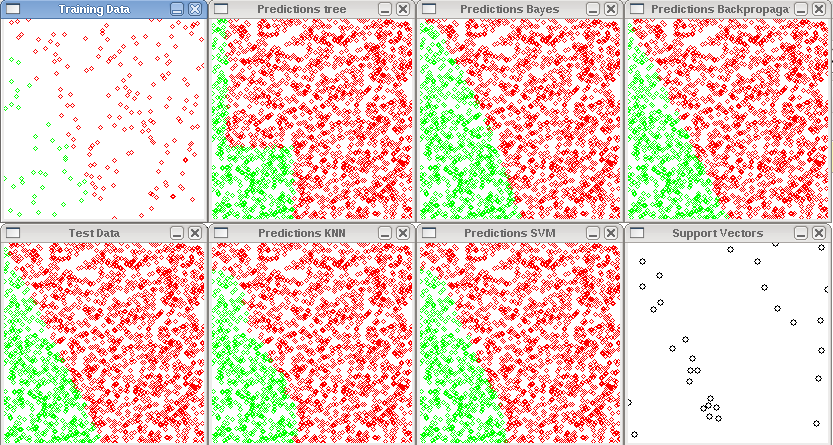
\includegraphics[scale=0.4]{img/eval/2x.png}

\subsection{y = sin(10x)}

\begin{tabular}{|c|c|}
\hline
Predictor &	Accuracy\\ \hline\hline
Support Vector Machine &	0.913\\ \hline
Multi Layer Perceptron (2, 10, 15, 1) & 0.6855\\ \hline
k-Nearest-Neighbor (k = 3) & 0.9\\ \hline
Normal Bayes & 0.632\\ \hline
Decision Tree &	0.886\\ \hline
\end{tabular}

\subsubsection{Plot}
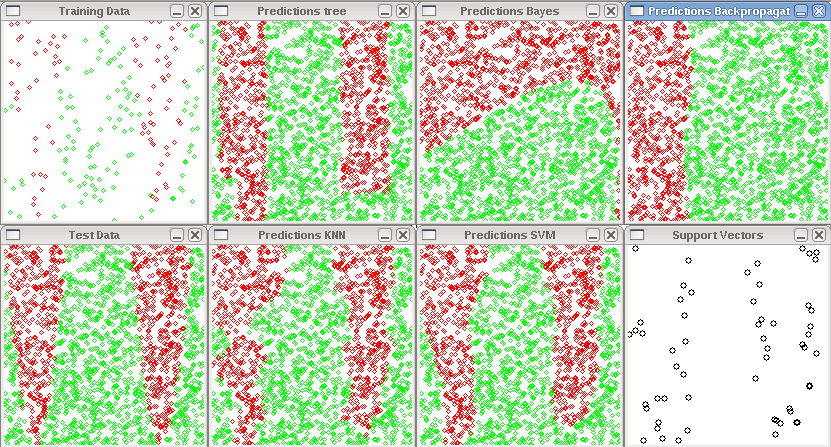
\includegraphics[scale=0.4]{img/eval/sin10x.png}

\subsection{y = tan(10x)}

\begin{tabular}{|c|c|}
\hline
Predictor &	Accuracy\\ \hline\hline
Support Vector Machine & 0.7815\\ \hline
Multi Layer Perceptron (2, 10, 15, 1) &	0.5115\\ \hline
k-Nearest-Neighbor (k = 3) & 0.8195\\ \hline
Normal Bayes &	0.542\\ \hline
Decision Tree &	0.9155\\ \hline
\end{tabular}

\subsubsection{Plot}
 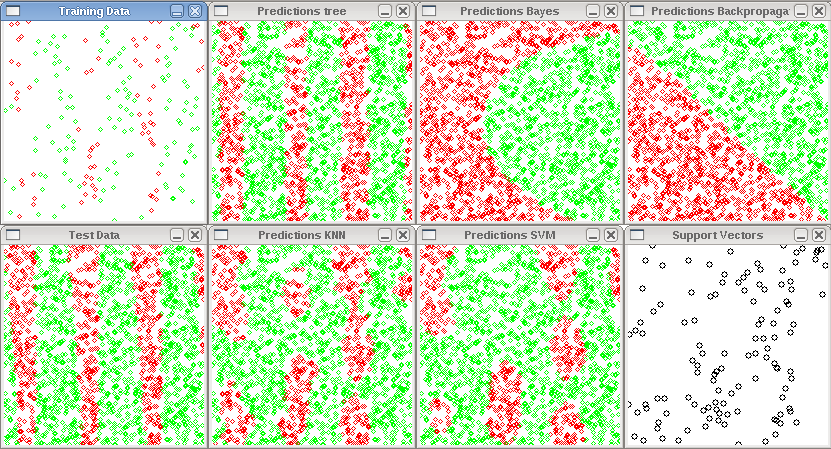
\includegraphics[scale=0.4]{img/eval/tan10x.png}


\appendix

% bibliography
\bibliography{bib/machinelearning}
\bibliographystyle{alphadin}

\end{document}
